\section{Theoretical Analysis}
\label{sec:analysis}

%foto parecida com slide 12
\par In this section we will make the theoretical analysis of our circuit. To do so, we will assume the ideal model for the 741 OP-AMP, were his gain is $A_v=\infty$, input impedance is $\infty$ and output impedance is $0$.

\par Using a feedback loop, we can stick $v_-$ to $v_+$ and make a non-inverting amplifier with gain: 
\begin{equation}
\frac A_{v1}{v_{O1}}{v_{I1}}=1+\frac{Z_3}{Z_4}
\end{equation}
Where, in our case, $Z_3=R_{31}+R_{32}+R_{33}=R_3$ and $Z_4=R_{41}||R_{42}=R_4$ are the resistive impedances. For this sub-circuit, the input and output impedances are, respectively, $Z_{I1}=\infty$ and $Z_{O1}=0$. 

\subsection{Transfer function and total gain}
%incluir foto parecida com slide 6, mas com os condensadores e resistencias externas

\par Now, we can substitute the previous sub-circuit with this model, and compute the transfer function for the complete circuit. 
\begin{equation}
v_O=\frac{Z_{C2}}{Z_{C2}+Z_{O1}+Z_{2}}A_{v1}v_{I1}=\frac{\frac{1}{C_2S}}{\frac{1}{C_2S}+R_2}(1+\frac{R_3}{R_4})v_{I1}
\end{equation}
\begin{equation}
v_{I1}=\frac{Z_{1}}{Z_{C1}+Z_{1}}v_{I}=\frac{R_1}{\frac{1}{C_1S}+R_1}v_{I}
\end{equation}

Then, the transfer function is given by:
\begin{equation}
T(S)=\frac{v_O}{v_I}=\frac{R_1C_1S}{1+R_1C_1S}(1+\frac{R_3}{R_4})\frac{1}{1+R_2C_2S}
\end{equation}
 Now, one can compute gain and phase from absolute value and phase of $T(S)$ and plot the frequency response for logarithmic vector of $\omega$:
 
 \begin{figure}[H] \centering
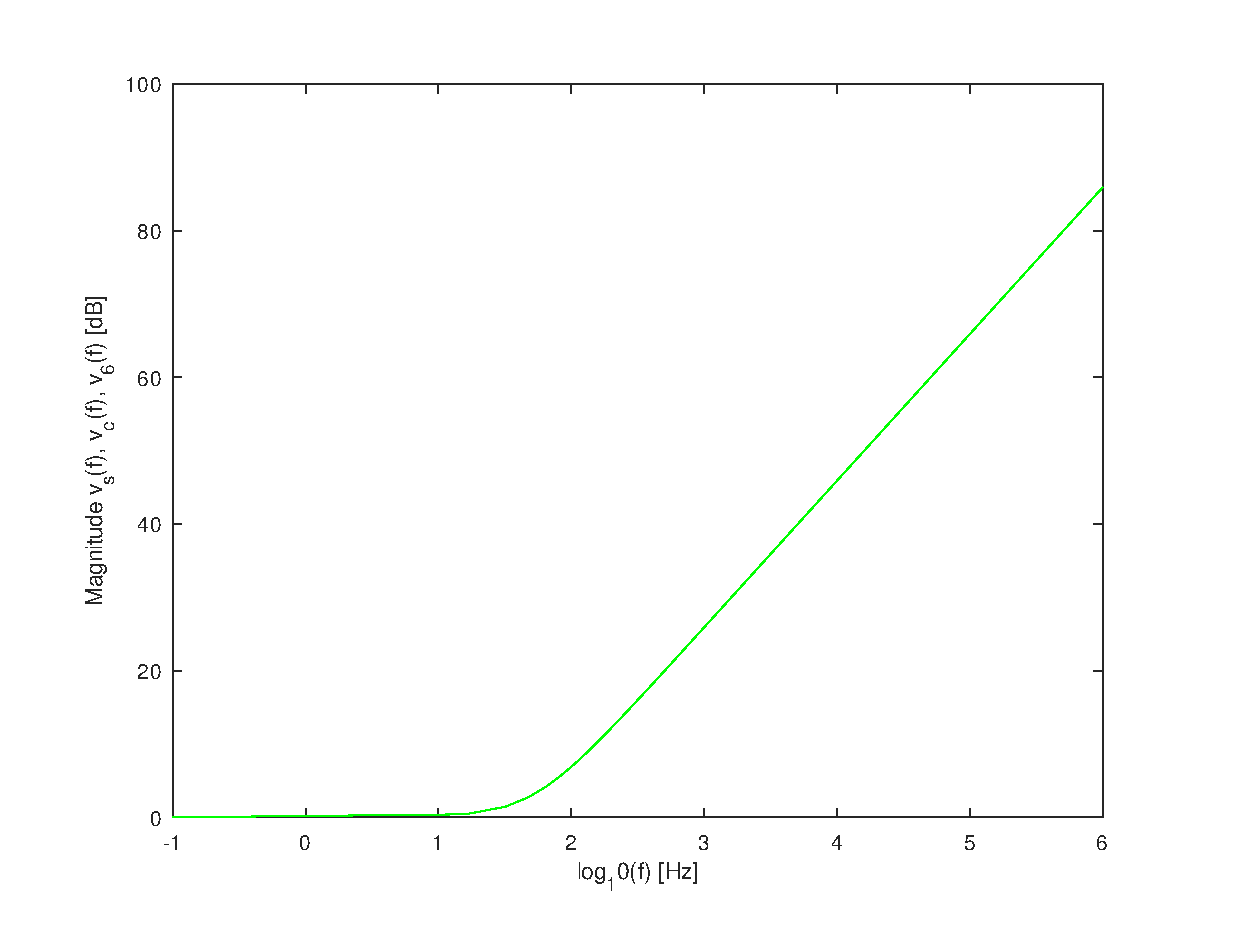
\includegraphics[width=0.8 \linewidth]{freq_db.eps}
\caption{Gain response to frequency (dB).}
\label{fig:gain}
\end{figure}

\begin{figure}[H] \centering
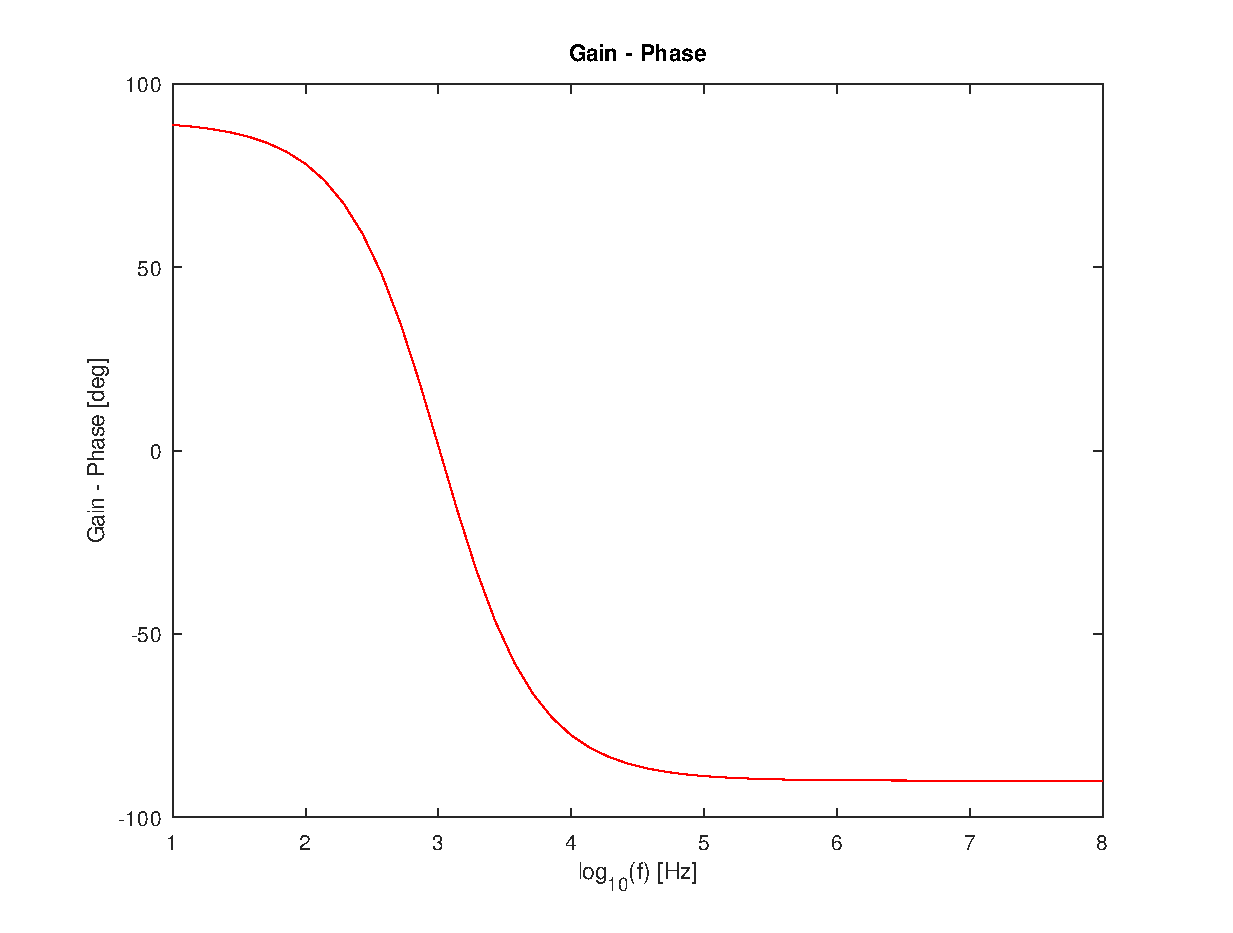
\includegraphics[width=0.8 \linewidth]{freq_p.eps}
\caption{Phase response to frequency (deg).}
\label{fig:phase}
\end{figure}
 
 \par As was suposed, we obtained a pass-band circuit, and the cut-off frequencies will be calculated in next chapter. This is achieved because, for low frequencies, the capacitors $C_1$ and $C_2$ behaves like open circuits, with high complex impedances, and it behaves like a short circuit for high frequencies. Therefore, $C_1$ will be a open circuit for low frequencies, the voltage that enters in the OP-AMP will be $v_{I1}\approx 0$ and $v_{O}\approx 0$, leaving the gain very low. In the other hand, for high, frequencies $C_2$ it's a short circuit and there will be no voltage drop in the capacitor, so $v_O\approx 0$ again.
 
 \subsection{Central frequency}
 \par From the poles of the transfer function, we obtain the lower and upper cut-off frequencies, respectively, $f_L$ and $f_H$.
 \begin{equation}
 f_L=\frac{1}{2\pi R_1C_1}
 \end{equation}
 \begin{equation}
 f_H=\frac{1}{2\pi R_2C_2}
 \end{equation}
 \par Then, we can compute the central frequency $f_0$ as a geometric mean of $f_L$ and $f_H$.
 \begin{equation}
 f_0=\sqrt{f_Lf_H}
 \end{equation}
 
 \par Next table shows the theoretical values for the cut-off and central frequencies.
 %tabela com cutoff
 \begin{table}[H]
    \centering
    \begin{tabular}{|l|r|}
    \hline    
    {\bf Name} & {\bf Value} \\ \hline
    \input{../mat/freq.tex}
    \end{tabular}
     \caption{Cut-off and central frequencies (Hz).}
    \label{tab:freq}
  \end{table}

 
 
 \subsection{Input and output impedances}
 %por ref a imagem
 \par To compute input impedance $Z_I$, seen from input voltage $v_I$, we substitute $Z_{I1}$ in the image \ref{} from is value $Z_{I1}=\infty$, therefore:
 
 \begin{equation}
 Z_I=Z_1+Z{C1}=R_1+\frac{1}{j2\pi f_0C_1}
 \end{equation}
\par For the output impedance $Z_{O}$, we set $v_I$ to $0$ and $Z_{O1}$ to his value $Z_{O1}=0$.
\begin{equation}
Z_O=R_2||C_2=\frac{1}{j2\pi f_0C_2+\frac{1}{R_2}}
\end{equation}

\par The values obtained for the input and output impedances are given in the next table.

%tabela com impedancias
\begin{table}[H]
    \centering
    \begin{tabular}{|l|r|}
    \hline    
    {\bf Name} & {\bf Value} \\ \hline
    $Z_I$ & $1707.106781$ \\ \hline 
$Z_O$ & $585.786438$ \\ \hline 

    \end{tabular}
     \caption{Input and output impedances.}
    \label{tab:freq}
  \end{table}



  
 


 
 
